%\begin{figure}
%  \begin{center}
%    \includegraphics[angle=0,width=0.7\textwidth]{figs/kin_flat.eps}
%    \caption{\label{KIN} Kinematic coverage.  Specific beam energies and angles
%    are detailed in Table~\ref{RATES}.~~  Dashed lines represent  the
%    interpolation to constant $Q^2$.
%     }
%  \end{center}
%\end{figure}
%
%%\begin{figure}
%\begin{center}
%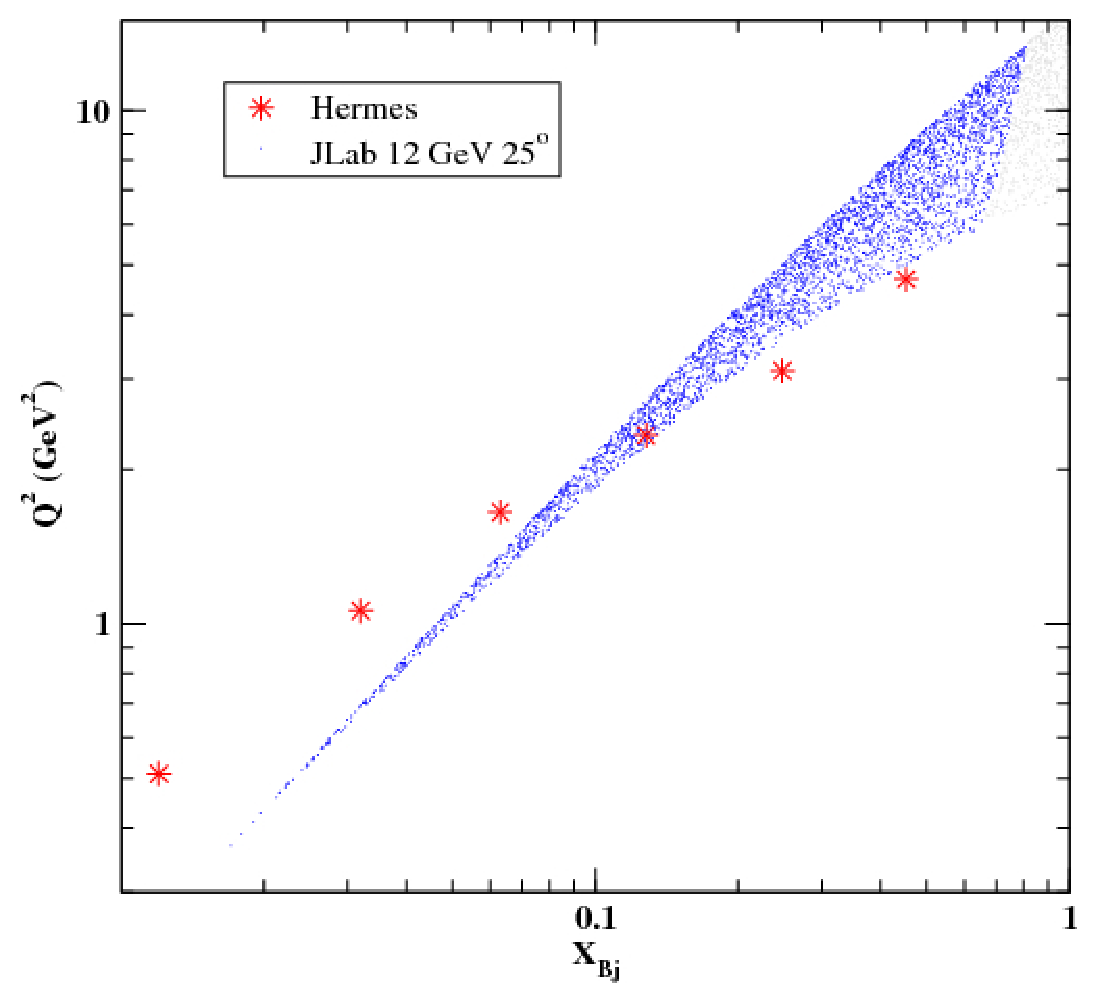
\includegraphics[width=0.425\textwidth]{figs/b1_kin_flat}
%\hspace{0.5cm}
%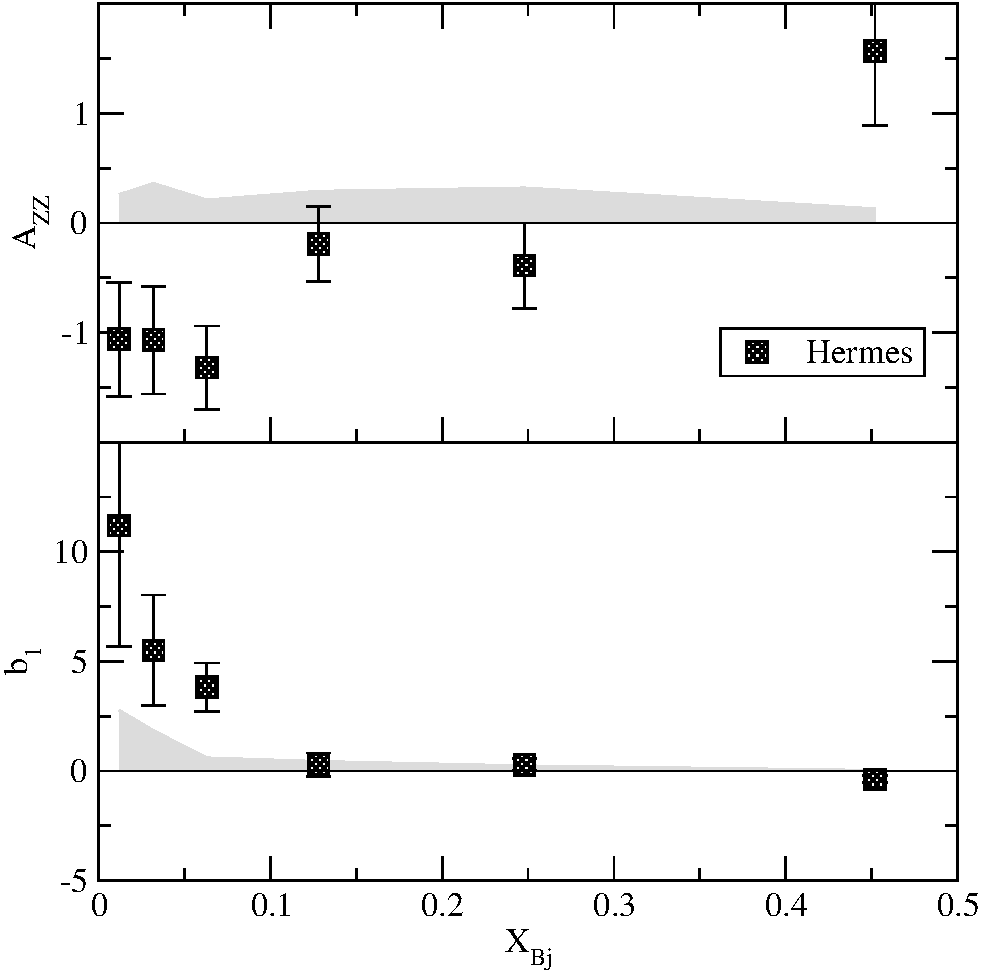
\includegraphics[width=0.39\textwidth]{figs/hermes_azz}
%\caption{\label{B1}
%{\bf Left: }
%Kinematic coverage for 12 GeV beam and Big Bite at $25^\circ$ compared to Hermes kinematic
%coverage.
%{\bf Right:} Data from Hermes\cite{Airapetian:2005cb}.
%}
%\end{center}
%\end{figure}

%
We will measure the deuteron tensor asymmetry $A_{zz}$ and extract the leading twist tensor structure 
function $b_1$ for $0.05<x<0.60$, $1.0<Q^2<5.0$ GeV$^2$ and $W \ge 2.0$ GeV. Fig.~\ref{kincov} 
shows the kinematic coverage available at JLab utilizing an 11 GeV beam, and the Hall A SoLID 
spectrometer. 

\begin{figure}[h]
\begin{center}
\includegraphics[width=0.6\textwidth]{figs/solid/cov_solid.eps}
\caption{\label{kincov} Kinematic coverage for 11 GeV beam in Hall A using the SoLID spectrometer.}
\end{center}
\end{figure}

The polarized target considered in this letter-of-intent is the solid lithium deuteride (LiD) 
since it has a better dilution factor than ND$_3$. The vector polarization, packing fraction and 
dilution used in the estimate of the rates are 55\%, 0.55 and 0.50 respectively. With an incident 
electron beam current of 100 nA, the expected deuteron luminosity is $2\times 10^{35}$ cm$^{-2}$s$^{-1}$. 
The acceptance of SoLID was assumed to be $\Delta\Omega = 1.43$ sr. 
The kinematics, physics rates\footnote{For this Letter-of-Intent, we took the rates expected from the Hall C 
HMS and scaled them to the SoLID acceptance $\Delta \Omega = 1.43$ sr. A detailed simulation will be
performed in a full proposal.}, projected statistical uncertainties of $A_{zz}$ and $b_1$ along with the time 
necessary to achieve this precision are summarized in Table~\ref{solidRATES}. The projected uncertainties 
are displayed in Fig.~\ref{solidPROJ}. Only rates with kinematics coverage of $W \ge 2.0$ GeV were computed. 
So 31 days of beam time is needed for production data. This time will be split equally between parallel and 
perpendicular running. About seven additional days will be needed for calibration, background study and 
configuration changes.


\begin{figure}
\begin{center}
\includegraphics[width=0.45\textwidth]{figs/solid/Azz_proj_lin_good.eps}
\hspace{0.5cm}
\includegraphics[width=0.45\textwidth]{figs/solid/xb1_proj_newmiller_lin_good.eps}
\caption{\label{solidPROJ}
{\bf Left: }
Projected precision of the tensor asymmetry $A_{zz}$ with 38 days of beam time. Also 
shown are the data from Hermes\cite{Airapetian:2005cb} and the calculation from Kumano~\cite{Kumano:2010vz}.
{\bf Right:} Corresponding projected precision of the tensor structure function $b_1$. In addition,
an updated calculation of Ref.~\cite{Miller:1989nc} from Miller is shown~\cite{Miller_tmp}. The black band
represents the systematic uncertainty.}
\end{center}
\end{figure}
%
\subsection{Overhead}
%
In order to calibrate the target NMR system, elastic scattering measurements will be performed at an 
incident energy of 2.2 GeV. Two days, including the energy pass change, should be sufficient. Measurements
of the dilution from the unpolarized materials contained in the target, and of the packing fraction due to 
the granular composition of the target material will be performed on a $^6$Li target and carbon target. 
A total of 8 hours of data will be needed. Target annealing and target material changes will be performed once 
a week. Table~\ref{solidOVHEAD} summarizes the expected overhead. The magnetic field of the target will be 
rotated from parallel to perpendicular configuration about once a week.
Approximately 7 additional days will be needed for calibration, background study and configuration changes.

\begin{table}[h]
\begin{center}
\caption{\label{solidOVHEAD}Summary of the overhead}
\begin{tabular}{c|ccc}\hline\hline
     ~                 &  time   & number &   total time \\
     ~                 &  (hrs)  &   ~    &    (hrs)     \\
\hline
elastic                &    ~    &   ~    &     48.0     \\
dilution               &    ~    &   ~    &     8.0      \\
configuration change   &   16    &   4    &     64.0     \\
beam energy meas.      &   2.0   &   2    &     4.0      \\
BCM calibration        &   1.0   &   2    &     2.0      \\
target annealing       &   2.5   &   4    &     10.0     \\
target material change &   4.0   &   4    &     16.0     \\
\hline\hline
\end{tabular}
\end{center}
\end{table}

\subsection{Background}
The pion background has not been estimated yet for this measurement, but should be comparable to other 
proposed DIS measurements with SoLID. A careful study of the background will be performed in a full 
proposal.

\begin{table}
\begin{center}
\caption{\label{solidRATES}Summary of the kinematics and physics rates using Hall A SoLID spectrometer for the measurement.}
\begin{tabular}{|ccc|cc|c|cc|cc|c|}\hline
 $<x>$  & $<Q^2>$      &  $<W>$  &    $P_0$    &    $\theta$  &  Rates & $A_{zz}$ & $\delta A_{zz}^{stat}$    & $b_1$  & $\delta b_1^{stat}$ & time   \\
  ~     & (GeV)$^2$  & (GeV) & (GeV)  &     (deg.)  &   (kHz)  & $\times 10^{-2}$ & $\times 10^{-2}$ &  $\times 10^{-2}$ & $\times 10^{-2}$    & (hours) \\
\hline\hline
 0.05 &   1.0 &    4.5 &   0.82 &   19.1 &   0.40 & -0.98 &  0.20 &  3.4  & 0.68  &   378 \\
 0.10 &   1.5 &    3.8 &   3.37 &   11.5 &   4.52 & -0.85 &  0.17 &  1.7  & 0.34  &    44 \\
 0.15 &   2.0 &    3.5 &   4.22 &   11.9 &   5.58 & -0.51 &  0.10 &  0.71 & 0.14  &   100 \\
 0.20 &   2.0 &    3.0 &   5.91 &   10.1 &  15.07 & -0.14 & 0.087 &  0.15 & 0.092 &    51 \\
 0.25 &   2.0 &    2.6 &   6.93 &    9.3 &  31.60 &  0.19 & 0.094 & -0.16 & 0.078 &    21 \\
 0.30 &   2.5 &    2.6 &   6.76 &   10.5 &  14.69 &  0.48 & 0.097 & -0.31 & 0.061 &    42 \\
 0.35 &   2.5 &    2.4 &   7.37 &   10.1 &  23.19 &  0.75 &  0.15 & -0.37 & 0.073 &    11 \\
 0.40 &   3.0 &    2.3 &   7.18 &   11.2 &  10.81 &  0.99 &  0.20 & -0.35 & 0.071 &    14 \\
 0.45 &   3.0 &    2.2 &   7.61 &   10.9 &  14.79 &  1.2  &  0.24 & -0.32 & 0.064 &     7 \\
 0.50 &   3.5 &    2.1 &   7.44 &   11.9 &   8.19 &  1.4  &  0.28 & -0.26 & 0.051 &     9 \\
 0.55 &   4.5 &    2.2 &   6.84 &   14.1 &   2.62 &  1.6  &  0.31 & -0.18 & 0.037 &    23 \\
 0.60 &   5.0 &    2.1 &   6.76 &   14.9 &   1.46 &  1.7  &  0.33 & -0.13 & 0.025 &    36 \\
\hline\hline
\end{tabular}
\end{center}
\end{table}

\subsection{Experimental Method}
Following Ref.~\cite{Hoodbhoy:1988am} it is possible to measure the asymmetry $A_{zz}$ by 
taking the difference of parallel and perpendicular cross sections with unpolarized beam:
\begin{eqnarray}
\frac{\frac{d^2\sigma_{\parallel}}{d\Omega dE'} - \frac{d^2\sigma_{\perp}}{d\Omega dE'}}
{\frac{d^2\sigma_{\parallel}}{d\Omega dE'} + 2 \frac{d^2\sigma_{\perp}}{d\Omega dE'}} = 
- \frac{1}{2} (1 - \frac{3}{2} H^2) A_{zz},
\label{para-perp}
\end{eqnarray}
%
where $H^2=(P+2)/3$ is the target spin projection along the beam and $P$ is the target polarization.
The polarized cross sections $d^2\sigma_{\parallel}/d\Omega dE'$ and $d^2\sigma_{\perp}/d\Omega dE'$ 
can be extracted from data collected by scattering an unpolarized electron beam off a spin-1 target 
polarized longitudinally and perpendicularly to the electron beam direction. 
The tensor structure function $b_1$ can then be extracted as follows:
\begin{eqnarray}
\frac{b_1}{F_1} = - \frac{3}{2} A_{zz}
\label{Azz}
\end{eqnarray}

From Eq.~\ref{para-perp}, the beam time needed to achieve an absolute uncertainty 
of $\delta A_{zz}$ can be deduced and is expressed as follows:
\begin{eqnarray}
T = \frac{32}{9 P_{zz}^2} \frac{1}{R_D~f~(P_{zz}~\delta A_{zz})^2}
\label{time-eq2}
\end{eqnarray}

with $R_D$ is the deuteron rate, $f$ the dilution factor and $P_{zz}$ the tensor polarization.

\subsection{Systematic Uncertainties}

In this Letter-of-Intent, we consider using a model for the unpolarized structure function
$F_1$ needed to extract $b_1$ from Eq.~\ref{xsmeth}. So an additional systematic uncertainty 
will have to be taken into account in the extraction of $b_1$ from the $A_{zz}$ measurement.

\begin{table}
\begin{center}
\begin{tabular}{|cc|}\hline
Polarimetry                  &   8\%   \\
Dilution/packing fraction    &   5\%   \\
Computer deadtime            &  0.5\%  \\
Charge measurement           &  0.5\%  \\
Energy measurement           &  0.05\% \\
Radiative corrections        &   5\%   \\         
\hline
Total Systematic Uncertainty &  11\%   \\
\hline
\end{tabular}
\caption{\label{sys}Relative systematic uncertainties.}
\end{center}
\end{table}

\subsection{Alternate Methodology}

In addition to the experimental approach considered in this Letter-of-Intent, we 
 have two other options which we will explore further in preparation for a full proposal: 
\begin{enumerate}
 \item measuring the tensor structure function $b_1$ with a longitudinally polarized target
using the cross section method suggested in Ref.~\cite{Hoodbhoy:1988am};
 \item measuring the tensor asymmetry $A_{zz}$ using the HERMES method~\cite{Riedl:2005jq}, 
with only a longitudinally polarized target.
\end{enumerate}
We are also exploring other forms of accessing $A_{zz}$ that don't rely on $A_2^d$ 
being negligible, like HERMES assumed.
